%Template pembuatan proposal skripsi.
\documentclass{jtetiskripsi}

%-----------------------------------------------------------------
%Disini awal masukan untuk data proposal skripsi
%-----------------------------------------------------------------
\titleind{PENGEMBANGAN GATEWAY BERBASIS EMBEDDED DEVICE UNTUK INTEROPERABILITAS JARINGAN SENSOR NIRKABEL DAN PROTOKOL INTERNET}

\fullname{GUNTUR DHARMA PUTRA}

\idnum{09/284593/TK/35393}

\approvaldate{13 November 2013}

\degree{Sarjana Teknik Elektro}

\yearsubmit{2013}

\program{Teknik Elektro}

\dept{Teknik Elektro dan Teknologi Informasi}

\firstsupervisor{Sigit Basuki Wibowo, S.T., M.Eng.}
\firstnip{1976 0501 2002 12 1 002}

\secondsupervisor{Bimo Sunarfri Hantono, S.T., M.Eng.}
\secondnip{1977 0131 2002 12 1 003}


%-----------------------------------------------------------------
%Disini akhir masukan untuk data proposal skripsi
%-----------------------------------------------------------------

\begin{document}

\cover

\approvalpage

%-----------------------------------------------------------------
%Disini awal masukan Acknowledment
%-----------------------------------------------------------------
\acknowledgment
\begin{flushright}
\emph{Karya sederhana ini kupersembahkan \\
buat Bapak, Ibu,\\dan Adik tercinta}
\end{flushright}

%-----------------------------------------------------------------
%Disini awal masukan untuk Prakata
%-----------------------------------------------------------------
\preface
Segala puji dan syukur semata-mata hanya untuk Allah SWT, karena atas segala
rahmat, hidayah dan bantuan-Nya jualah maka akhirnya Tesis dengan judul
Analisis Teoretis Pemantulan dan Pembiasan Gelombang Elektromagnet Pada
Bahan Magnetik Non Linear Orde Dua ini telah selesai penulis susun.

Telah banyak bantuan yang penulis peroleh selama dalam penulisan Tesis ini
, untuk itu tak lupa penulis ucapkan terima kasih yang sebesar-besarnya
kepada:
\begin{enumerate}
\item{Bapak dan Mama yang selama ini telah sabar membimbing dan mendoakan
penulis tanpa kenal untuk selama-lamanya,}
\item{Prof. Drs. H. Muslim, Ph. D, selaku Pembimbing Utama, yang telah
memberikan ilmunya kepada penulis serta dengan penuh kesabaran membimbing penulis,}
\item{Drs. Kamsul Abraha, Ph. D, selaku Pembimbing Pendamping yang telah
memberikan inspirasi kepada penulis,} 
\item{Dr. Pekik Nurwantoro dan Dr. rer. nat. M. Farchani Rasyid
yang telah memperkenalkan sistem operasi LINUX dan \LaTeX{} kepada penulis serta
memberikan bimbingan penggunaan \LaTeX{} tersebut dengan sabar,} 
\item{Segenap staf dan karyawan di jurusan Fisika FMIPA UGM, yang telah
banyak bekerjasama dengan penulis selama belajar di FMIPA UGM,} 
\item{Sahabat saya M. Rizal Ginanjar, yang selalu bersedia membantu penulis ketika
menyelesaikan masalah-masalah komputer.} 
\end{enumerate}

Tesis ini tentunya tidak lepas dari segala kekurangan dan kelemahan, untuk itu
segala kritikan dan saran yang bersifat membangun guna kesempurnaan Tesis ini
sangat diharapkan. Semoga tesis ini dapat bermanfaat bagi kita semua dan lebih
khusus lagi bagi pengembagan ilmu fisika.

\begin{tabular}{p{7.5cm}c}
&Yogyakarta, 12 Mei 1994\\
&\\
&\\
&Penulis
\end{tabular}

%-----------------------------------------------------------------
%Disini akhir masukan untuk muka skripsi
%-----------------------------------------------------------------

\tableofcontents
\addcontentsline{toc}{chapter}{DAFTAR ISI}
\listoftables
\addcontentsline{toc}{chapter}{DAFTAR TABEL}
\listoffigures
\addcontentsline{toc}{chapter}{DAFTAR GAMBAR}

%-----------------------------------------------------------------
%Disini awal masukan Intisari
%-----------------------------------------------------------------
\begin{abstractind}
Penggunaan \emph{Wireless Sensor Network} (WSN) untuk gedung dan perumahan semakin populer karena dapat dimanfaatkan untuk berbagai kepentingan seperti \emph{home automation} dan \emph{home surveillance}. Oleh karena itu, untuk meningkatkan fleksibilitas penggunaan WSN, diperlukan sistem pengendalian yang dapat dikendalikan secara jarak jauh. Padahal pada umumnya, WSN dikendalikan oleh sebuah pengendali utama berada di sekitar tempat WSN itu berada.

Penelitian ini mengusulkan integrasi dari WSN dengan \emph{Internet Protocol} (IP) yang memungkinkan WSN dapat dikendalikan dimanapun dan dengan apapun asalkan masih terhubung dengan jaringan internet. Penelitian ini memanfaatkan infrastruktur jaringan data yang sangat populer dan terhubung ke internet, yaitu jaringan area lokal nirkabel atau dikenal dengan nama WiFi. Salah satu perangkat utama dalam jaringan WiFi adalah \emph{Access Point} (AP) yang berfungsi sebagai koordinator simpul. Selain itu, AP juga berfungsi sebagai gateway yang menghubungkan berbagai piranti yang terhubung padanya ke internet. Oleh karena itu, penelitian ini akan mengembangkan perangkat lunak yang akan ditanamkan ke dalam AP sehingga menjadikan AP mempunyai kemampuan sebagai gateway untuk kedua jaringan WiFi dan beberapa protokol WSN ke dalam jaringan internet.


\bigskip
\textbf{Kata kunci} : \emph{wireless sensor network}, \emph{internet protokol}, WiFi, interoperabilitas.
\end{abstractind}

\begin{abstracteng}
Penggunaan \emph{Wireless Sensor Network} (WSN) untuk gedung dan perumahan semakin populer karena dapat dimanfaatkan untuk berbagai kepentingan seperti \emph{home automation} dan \emph{home surveillance}. Oleh karena itu, untuk meningkatkan fleksibilitas penggunaan WSN, diperlukan sistem pengendalian yang dapat dikendalikan secara jarak jauh. Padahal pada umumnya, WSN dikendalikan oleh sebuah pengendali utama berada di sekitar tempat WSN itu berada.

Penelitian ini mengusulkan integrasi dari WSN dengan \emph{Internet Protocol} (IP) yang memungkinkan WSN dapat dikendalikan dimanapun dan dengan apapun asalkan masih terhubung dengan jaringan internet. Penelitian ini memanfaatkan infrastruktur jaringan data yang sangat populer dan terhubung ke internet, yaitu jaringan area lokal nirkabel atau dikenal dengan nama WiFi. Salah satu perangkat utama dalam jaringan WiFi adalah \emph{Access Point} (AP) yang berfungsi sebagai koordinator simpul. Selain itu, AP juga berfungsi sebagai gateway yang menghubungkan berbagai piranti yang terhubung padanya ke internet. Oleh karena itu, penelitian ini akan mengembangkan perangkat lunak yang akan ditanamkan ke dalam AP sehingga menjadikan AP mempunyai kemampuan sebagai gateway untuk kedua jaringan WiFi dan beberapa protokol WSN ke dalam jaringan internet.


\bigskip
\textbf{Kata kunci} : \emph{wireless sensor network}, \emph{internet protokol}, WiFi, interoperabilitas.
\end{abstracteng}
%-----------------------------------------------------------------
%Disini akhir masukan Intisari
%-----------------------------------------------------------------

%-----------------------------------------------------------------
%Disini awal masukan untuk Bab
%-----------------------------------------------------------------
%-------------------------------------------------------------------------------
% 								BAB I
% 							LATAR BELAKANG
%-------------------------------------------------------------------------------

\chapter{LATAR BELAKANG}

\section{Latar Belakang Masalah}
Lorem ipsum dolor sit amet, consectetuer adipiscing elit, sed diam nonummy nibh euismod tincidunt ut laoreet dolore magna aliquam erat volutpat. Ut wisi enim ad minim veniam, quis nostrud exerci tation ullamcorper suscipit lobortis nisl ut aliquip ex ea commodo consequat. Duis autem vel eum iriure dolor in hendrerit in vulputate velit esse molestie consequat, vel illum dolore eu feugiat nulla facilisis at vero eros et accumsan et iusto odio dignissim qui blandit praesent luptatum zzril delenit augue duis dolore te feugait nulla facilisi. Nam liber tempor cum soluta nobis eleifend option congue nihil imperdiet doming id quod mazim placerat facer possim assum.\cite{wibowo2013wireless,Raluca2008}.

\section{Rumusan Masalah}
Habeo perfecto in sea. Ea deleniti gloriatur pri, paulo mediocrem incorrupte sea ei. Ad mollis scripta per. Incorrupte sadipscing ne mel. Mel ex nonumy malorum epicurei. Ne per tota mollis suscipit. Ullum labitur vim ut, ea dicit eleifend dissentias sit. Duis praesent expetenda ne sed. Sit et labitur albucius elaboraret. Ceteros efficiantur mei ad. Hendrerit vulputate democritum est at, quem veniam ne has, mea te malis ignota volumus.


\section{Batasan Masalah}
Batasan masalah pada penelitian ini adalah:
\begin{enumerate}
\item Penelitian ini difokuskan pada interoperabilitas beberapa \emph{vendor} WSN dan protokol Internet.
\item Tipe WSN yang digunakan dalam penelitian ini dibatasi dua buah.
\item Pengujian yang dilakukan hanya sebatas eksperimen dalam lingkup laboratorium.
\item Purwarupa yang dihasilkan akan diimplementasikan pada sebuah \emph{Access Point} (AP).
\end{enumerate}


\section{Tujuan Penelitian}
Eros reprimique vim no. Alii legendos volutpat in sed, sit enim nemore labores no. No odio decore causae has. Vim te falli libris neglegentur, eam in tempor delectus dignissim, nam hinc dictas an.


\section{Manfaat Penelitian}
Pro omnium incorrupte ea. Elitr eirmod ei qui, ex partem causae disputationi nec. Amet dicant no vis, eum modo omnes quaeque ad, antiopam evertitur reprehendunt pro ut. Nulla inermis est ne. Choro insolens mel ne, eos labitur nusquam eu, nec deserunt reformidans ut. His etiam copiosae principes te, sit brute atqui definiebas id.

Et affert civibus has. Has ne facer accumsan argumentum, apeirian hendrerit persequeris pro ex. Suscipit vivendum sensibus mea at, vim ei hinc numquam, at dicit timeam dissentiet mel. At patrioque intellegebat sea, error argumentum dissentias sea in.


\section{Keaslian Penelitian}
No per amet modo comprehensam, duo dolor dignissim ex, ancillae corrumpit intellegam vix te. Mel utinam signiferumque no, ex nec accusam accumsan. Et per inermis posidonium, qui et ornatus epicuri pertinax. In homero commodo usu, vel te habemus fuisset, id nec periculis sententiae efficiendi. Oblique sanctus intellegat at cum.


\section{Sistematika Penulisan}
\noindent
\textbf{BAB I : PENDAHULUAN}

Pada bab ini dijelaskan latar belakang, rumusan masalah, batasan, tujuan, manfaat, keaslian penelitian, dan sistematika penulisan.\\

\noindent
\textbf{BAB II : TINJAUAN PUSTAKA DAN LANDASAN TEORI}

Pada bab ini dijelaskan teori-teori dan penelitian terdahulu yang digunakan sebagai acuan dan dasar dalam penelitian.\\

\noindent
\textbf{BAB III : METODOLOGI PENELITIAN}

Pada bab ini dijelaskan metode yang digunakan dalam penelitian meliputi langkah kerja, pertanyaan penilitian, alat dan bahan, serta tahapan dan alur penelitian.\\

\noindent
\textbf{BAB IV : HASIL DAN PEMBAHASAN}

Pada bab ini dijelaskan hasil penelitian dan pembahasannya.\\

\noindent
\textbf{BAB V : KESIMPULAN DAN SARAN}

Pada bab ini ditulis kesimpulan akhir dari penelitian dan saran untuk pengembangan penelitian selanjutnya.\\

% Baris ini digunakan untuk membantu dalam melakukan sitasi
% Karena diapit dengan comment, maka baris ini akan diabaikan
% oleh compiler LaTeX.
\begin{comment}
\bibliography{daftar-pustaka}
\end{comment}


%-------------------------------------------------------------------------------
%                            BAB II
%               TINJAUAN PUSTAKA DAN DASAR TEORI
%-------------------------------------------------------------------------------

\chapter{TINJAUAN PUSTAKA DAN DASAR TEORI}                

\section{Tinjauan Pustaka}
  Secara umum, cara untuk menghubungkan WSN dengan jaringan internet dapat dikelompokkan menjadi dua. Cara pertama adalah menggunakan gateway dan cara yang kedua adalah dengan menggunakan simpul sensor yang sudah dilengkapi dengan protokol internet. Cara yang lebih mudah ditempuh adalah dengan cara yang pertama karena pengubahan yang dilakukan relatif tidak terlalu besar. Sedangkan cara yang kedua akan menemui banyak kendala terutama pada WSN yang sudah terpasang karena harus dilakukan penggantian tiap simpul sensor.

  Salah satu usaha untuk mengintegrasikan jaringan WSN dengan jaringan WiFi menggunakan gateway misalnya dilakukan pada penelitian. Pada riset tersebut pengintegrasian dilakukan dengan sebuah komputer yang didedikasikan untuk keperluan tertentu. Penggunaan komputer khusus ini adalah hardware-solution yang membutuhkan biaya dan kerumitan sistem.

  Riset pada juga menawarkan pengintegrasian dengan jaringan IP. Namun demikian di dalam riset ini diperlukan perubahan yang signifikan jika konfigurasi jaringan sensor nirkabel sudah terpasang. Simpul sensor yang digunakan harus diganti dengan simpul sensor yang mendukung IP. Hal ini jelas akan memakan biaya yang cukup besar dan tidak praktis untuk dilakukan. Terlebih lagi jika jumlah sensor yang terpasang jumlahnya cukup banyak.

  Riset pada sudah berhasil mengembangkan sebuah AP menjadi gateway yang dapat digunakan untuk menghubungkan sebuah protokol WSN dengan jaringan IP. Protokol WSN yang digunakan adalah protokol dari IQRF. Penelitian tersebut kemudian dilanjutkan dengan penelitian yang sudah diterapkan dalam sistem domotic.

\section{Landasan Teori}
  \subsection{\emph{Wireless Sensor Network}}
    Jaringan sensor nirkabel (Wireless Sensor Network, WSN) adalah jaringan simpul sensor otonom yang terdistribusi digunakan untuk memonitor kondisi fisik atau lingkungan misalnya suhu, suara, getaran, kelembaban, dan lain-lain. Selain itu, tidak menutup kemungkinan untuk menambahkan fungsi tambahan pada setiap simpul misalnya port masukan/keluaran (I/O port) yang terdapat dalam setiap simpul dihubungkan dengan aktuator sehingga dapat digunakan untuk mengendalikan piranti elektrik atau elektronis.

    Secara umum, WSN dapat diilustrasikan seperti Gambar \ref{wsn}. Pada gambar tersebut terlihat adanya beberapa simpul yang diwakili dengan titik berukuran kecil dan satu buah simpul yang diwakili dengan titik berukuran lebih besar. Titik yang berukuran kecil mewakili simpul sensor sedangkan titik yang berukuran besar mewakili gateway yang berfungsi menghubungkan jaringan sensor nirkabel dengan pengendali utama yang dalam gambar tersebut diwakili oleh sebuah komputer. Contoh sebuah simpul dari IQRF ditunjukkan pada Gambar \ref{iqrf}.

      \begin{figure}[ht!]
        \centering
          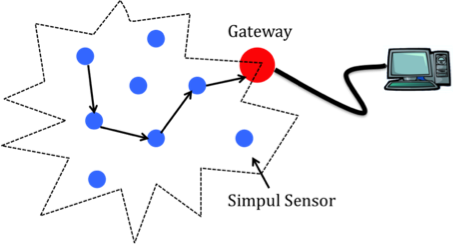
\includegraphics{gambar/wsn}
          \caption{Jaringan sensor nirkabel.}
          \label{wsn}
      \end{figure}

    Pada umumnya, WSN adalah jaringan yang berdiri sendiri. Untuk menghubungkan WSN dengan jaringan yang lain misalnya jaringan internet, maka salah satu cara adalah dengan membangun gateway WSN yang mampu menjembatani perbedaan protokol yang ada pada WSN dan jaringan internet. Cara tersebut adalah cara yang ditempuh dalam penelitian ini karena lebih mudah dilakukan dibandingkan dengan cara yang lain seperti sudah dijelaskan pada Bab Tinjauan Pustaka.

      \begin{figure}[ht!]
        \centering
          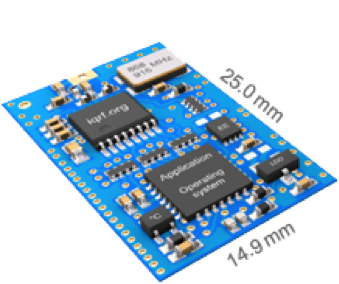
\includegraphics{gambar/iqrf}
          \caption{Contoh sebuah simpul sensor IQRF.}
          \label{iqrf}
      \end{figure}

    Sementara itu, jaringan WiFi sebagai jaringan lokal nirkabel yang digunakan untuk komunikasi data dalam suatu area lokal dan sudah tersebar di berbagai tempat. Lokal yang dimaksud disini adalah area yang tidak terlalu luas yaitu dengan radius sekitar 20m atau dalam sebuah gedung. Untuk membangun jaringan lokal menggunakan WiFi, perangkat utama yang digunakan adalah Access Point (AP). AP adalah piranti yang akan menjadi koordinator dalam jaringan lokal jika diinginkan topologi bintang (star) seperti diilustrasikan pada Gambar \ref{star}.

      \begin{figure}[ht!]
        \centering
          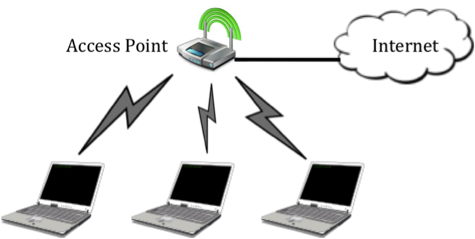
\includegraphics{gambar/star}
          \caption{Jaringan bintang menggunakan WiFi.}
          \label{star}
      \end{figure}

    Gambar \ref{star} memberi ilustrasi sebuah jaringan WiFi yang terdiri dari tiga buah komputer dan satu buah AP yang terhubung ke jaringan internet. Dengan konfigurasi tersebut, semua komputer yang ada di dalam jaringan WiFi dapat berkomunikasi dengan internet dengan aturan yang ditentukan oleh AP.

    Jika dilihat lebih dalam lagi, AP ini sebenarnya adalah piranti tertanam (embedded device) yang didalamnya sudah terdapat pusat pengolahan utama, memory, dan penyimpanan (storage). Dengan kenyataan inilah maka AP mempunyai potensi untuk menjagi gateway bagi jaringan WiFi dan WSN ke jaringan internet. Untuk mengembangkan aplikasi yang akan ditanamkan ke dalam AP, maka diperlukan sistem operasi yang sesuai untuk AP.

  \subsection{IQRF}
    IQRF adalah teknologi komunikasi nirkabel berbasis paket melalui frekuensi radio dalam pita frekuensi sub-GHz. Teknologi ini dimaksudkan untuk penggunaan umum saat konektivitas nirkabel dibutuhkan, entah \emph{point to point} atau jaringan yang kompleks. fungsionalitas lengkapnya bergantung semata-mata pada aplikasi berbahasa C yang ditulis oleh pengguna.

    Peranti kominikasi dasar dari IQRF adalah sebuah modul pancar-rima termasuk unit mikrokontroler dengan sistem operasi tertanam yang mengimplementasikan lapisan \emph{link} dan lapisan jaringan yang mendukung jaringan jala (\emph{mesh}) dengan protokol IQMESH. Tidak ada tingkat komunikasi yang lebih tinggi seperti lapisan \emph{transport} yang termasuk kedalam teknologi ini.

    Fitur-fitur yang dimiliki antara lain:
      \begin{itemize}
        \item Kecepatan, daya, dan ukuran data yang rendah,
        \item RF yang berbasis paket data, maksimal 128 Byte per paket,
        \item pita frekuensi sub-GHz (868 MHz, 916 MHz, dst.), \emph{multichannel}, dan modulasi FSK,
        \item \emph{bit rate} 1.2 kb/s – 86.2 kb/s,
        \item daya keluaran maksimal 20 mW,
        \item maksimal 65.000 peranti dalam satu jaringan,
        \item konsumsi daya yang rendah: 380 nA saat \emph{standby}, 25 µA saat menerima.
      \end{itemize}


  \subsection{XBee}
    XBee adalah sebuah merk dari Digi International untuk keluarga modul radio. XBee pertama diperkenalkan dalam merk MaxStream pada tahun 2005 yang berdasarkan pada standar IEEE 802.15.4-2003 untuk \emph{point to point} dan komunikasi bintang dalam \emph{baud rate} 250 kbit/s.

      \begin{figure}[ht!]
        \centering
          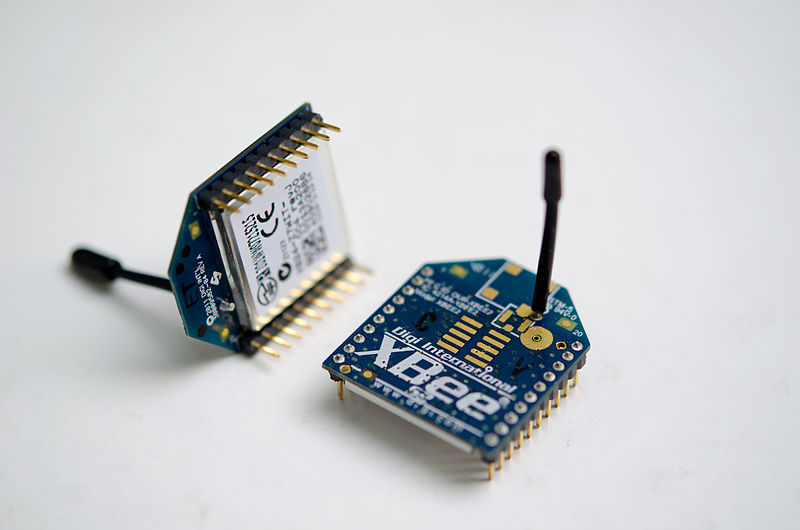
\includegraphics[width=0.5\textwidth]{gambar/xbee}
          \caption{Sepasang peranti XBee.}
          \label{xbee}
      \end{figure}

    Pada awalnya diperkenalkan dua model, yaitu 1mW XBee dan 100mW XBee-PRO. Sejak pertama kali diperkenalkan, beberapa buah XBee baru juga diperkenalkan dan semua XBee sekarang dipasarkan dengan merk Digi. Contoh peranti XBee dapat dilihat pada Gambar \ref{xbee}.

  \subsection{TCP/IP}
    Protokol internet adalah kumpulan protokol-protokol komunikasi yang digunakan dalam internet dan jaringan komputer sejenis, dan umumnya merupakan protokol yang paling populer untuk WAN. Pada umumnya hal ini dikenal dengan TCP/IP, karena protokol utamanya merupakan protokol jaringan pertama yang terstandarisasi. Terkadang hal ini dikenal dengan model DoD karena pengaruh ARPANET pada dekade 1970an.

    TCP/IP menyediakan konektivitas antar ujung yang menspesifikasikan bagaimana data harus diformat, dialamatkan, ditransmisikan, dirutekan, dan diterima di tujuan. TCP/IP memiliki empat layer abstraksi yang digunakan untuk mengurutkan semua protokol internet menurut jangkauan jaringan yang terlibat. Dari terendah sampai tertinggi, lapisan-lapisan tersebut adalah layer link, layer internet, layer transport, dan layer aplikasi.

  \subsection{\emph{Access Point}}
    \emph{Access Point}, disingkat AP, atau juga dikenal dengan istilah \emph{Wireless Access Point} adalah sebuah peranti yang memungkinkan peranti-peranti nirkabel untuk terkoneksi dengan jaringan kabel menggunakan Wi-Fi atau standar lain. AP biasanya terkoneksi dengan sebuah \emph{router} (melalui jaringan kabel) sebagai peranti yang berdiri sendiri, namun juga dapat menjadi bagian dalam komponen \emph{router} tersebut.

    Penggunaan secara korporat melibatkan beberapa AP ke dalam jaringan kabel dan menyediakan akses nirkabel ke LAN kantor. AP diatur dengan WLAN \emph{Controller} yang menangani pengaturan daya RF, kanal-kanal, autentikasi, dan keamanan.
    
    Sebuah \emph{hotspot} adalah aplikasi dari satu atau beberapa AP, di mana peranti dapat terhubung ke Internet dengan mudah. Konsep ini sudah menjadi hal yang umum di beberapa kota besar, di mana kombinasi dari warung kopi, perpustakaan, dan AP milik pribadi memungkinkan klien untuk terkoneksi dengan Internet. Koleksi dari \emph{hotspot} yang terkoneksi dapat disebut sebagai sebuah jaringan \emph{lili pad}.

  \subsection{Web Server}
    Web server dapat mengacu pada perangkat keras atau perangkat lunak yang membantu dalam penyampaian konten web yang dapat diakses melalui internet.

    Penggunaan web server yang paling umum adalah sebagai host untuk halaman web, walaupun ada beberapa penggunaan lain seperti game, media penyimpan data, atau penjalanan aplikasi perusahaan.


  \subsection{AJAX}
    AJAX adalah kelompok dari teknik-teknik pengembangan web yang digunakan pada klien untuk membuat aplikasi asinkron. Dengan AJAX, aplikasi web dapat mengirim dan menerima data dari sebuah server secara asinkron tanpa mengganggu tampilan dari halaman yang ada. Data dapat diambil menggunakan obyek XMLHttpRequest. Penggunaan XML tidak diperlukan, malahan JSON lebih sering digunakan, dan rekues tidak harus asinkron.

    AJAX bukanlah sebuah teknologi, tapi kelompok dari teknologi-teknologi. HTML dan CSS dapat digunakan dalam kombinasi untuk mark up dan informasi tampilan. DOM diakses oleh JavaScript untuk menampilkan dan mengijinkan pengguna untuk berinteraksi dengan informasi tertampil. JavaScript dan obyek XMLHttpRequest menyediakan sebuah metode untuk pertukaran data secara asinkron antara browser dan server untuk menghindari muat ulang halaman secara keseluruhan.


  \subsection{OpenWRT}
    OpenWRT adalah sebuah sistem operasi untuk \emph{embedded device} yang berbasis pada Linux kernel. OpenWRT pada umumnya digunakan dalam routing \emph{network traffic}. Komponen-komponen utamanya adalah Linux kernel, util-linux, uClibc dan BusyBox. Semua komponen sudah dioptimalkan dan dimampatkan untuk bisa muat dalam \emph{router} rumahan yang memiliki keterbatasan media penyimpan dan memori. OpenWRT dapat dikonfigurasikan melalui antarmuka \emph{command-line} (\emph{ash shell}), seperti dapat dilihat pada Gambar \ref{openwrt}, atau dengan antarmuka Web (LuCI). Terdapat kurang lebih 3.500 paket-paket perangkat lunak tambahan yang tersedia untuk diinstal melalui sistem manajemen paket \emph{opkg}.

      \begin{figure}[ht!]
        \centering
          
\includegraphics[width=10cm]{gambar/openwrt}
          \caption{Tampilan antarmuka \emph{command-line} OpenWRT versi \emph{BackFire}.}
          \label{openwrt}
      \end{figure}

    OpenWRT dapat berjalan pada router CPE (\emph{Customer Premised Equipment}), \emph{gateway} residensial, komputer saku (seperti Ben NanoNote), dan komputer jinjing. OpenWRT juga dapat berjalan pada komputer konvensional atau komputer dengan arsitektur x86. Banyak \emph{patch} dari kode sesumber berbasis OpenWRT yang diubah kedalam Linux kernel utama.

  \subsection{SSHFS}
    SSHFS (SSH Filesystem) adalah sebuah klien \emph{filesystem} untuk \emph{mount} dan berinteraksi dengan direktori dan arsip yang berlokasi pada server atau \emph{workstation}. Klien berinteraksi dengan server dengan SSH \emph{File Transfer Protocol} (SFTP), sebuah protokol jaringan yang menyediakan akses ke arsip, transfer arsip, dan fungsionalitas manajemen arsip melalui aliran data yang didesain sebagai ekstensi dari protokol SSH versi 2.0.

  \subsection{Bootstrap}
    Bootstrap adalah koleksi gratis dari alat-alat untuk membuat situs web dan aplikasi berbasis web. Bootstrap terdiri dari HTML dan contoh desain berbasis CSS untuk tipografi, borang, tombol, navigasi, komponen antarmuka lain, dan juga ekstensi JavaScript yang bersifat opsional.

    Bootstrap merupakan proyek paling populer pada GitHub, dan sudah digunakan oleh, diantaranya, NASA dan MSNBC.


%-------------------------------------------------------------------------------
%                            BAB III
%               		METODOLOGI PENELITIAN
%-------------------------------------------------------------------------------

\chapter{METODOLOGI PENELITIAN}

\section{Alat dan Bahan}
	Alat dan bahan yang digunakan pada penelitian ini terbagi atas perangkat keras dan perangkat lunak yang akan dijelaskan seperti berikut.

	\subsection{Perangkat Keras}
		Pro omnium incorrupte ea. Elitr eirmod ei qui, ex partem causae disputationi nec. Amet dicant no vis, eum modo omnes quaeque ad, antiopam evertitur reprehendunt pro ut. Nulla inermis est ne. Choro insolens mel ne, eos labitur nusquam eu, nec deserunt reformidans ut. His etiam copiosae principes te, sit brute atqui definiebas id.

		\vspace{-0.5cm}

		\begin{enumerate}[a.]
		\begin{singlespace}
		\itemsep0em
			\item Kit pancar-rima IQRF TR-53B (3 unit),
			\item Kit pengunduh program CK-USB-04 (1 unit),
			\item Kit pengembangan DK-EVAL-03 (2 unit),
			\item Kit pengembangan CK-EVAL-04 (1 unit),
			\item \emph{XBee 802.15.4 Radios (Series 1)} (3 unit),
			\item \emph{XBee Explorer USB Board} (1 unit),
			\item \emph{2 channel Relay Shield For Arduino (With XBee/BTBee interface)} (2 unit),
			\item Arduino Uno (2 unit),
			\item TP-LINK MR3020 (1 unit),
			\item Kabel USB ke Serial Prolific (1 unit).
		\end{singlespace}
		\end{enumerate}

	\subsection{Perangkat Lunak}
		Pro omnium incorrupte ea. Elitr eirmod ei qui, ex partem causae disputationi nec. Amet dicant no vis, eum modo omnes quaeque ad, antiopam evertitur reprehendunt pro ut. Nulla inermis est ne. Choro insolens mel ne, eos labitur nusquam eu, nec deserunt reformidans ut. His etiam copiosae principes te, sit brute atqui definiebas id.

		\vspace{-0.5cm}

		\begin{enumerate}[a.]
		\begin{singlespace}
		\itemsep0em
			\item Arduino for Mac OS X,
			\item CoolTerm,
			\item Driver FTDI for Mac OS X,
			\item PHP, MySQL, dan uHTTPd,
			\item Python dan pustaka PySerial,
			\item IQRF IDE v 2.08 for TR-53B,
			\item SSHFS,
			\item Sublime Text 3.
		\end{singlespace}
		\end{enumerate}

\section{Alur Penelitian}
	Consul graeco signiferumque qui id, usu eu summo dicunt voluptatum, nec ne simul perpetua posidonium. Eos ea saepe prodesset signiferumque. No dolore possit est. Mei no justo intellegebat definitiones, vis ferri lorem eripuit ad. Solum tritani scribentur duo ei, his an adipisci intellegat.

\section{Tahapan Pelaksanaan}
	Consul graeco signiferumque qui id, usu eu summo dicunt voluptatum, nec ne simul perpetua posidonium. Eos ea saepe prodesset signiferumque. No dolore possit est. Mei no justo intellegebat definitiones, vis ferri lorem eripuit ad. Solum tritani scribentur duo ei, his an adipisci intellegat.

\section{Jadwal Kegiatan}
	Quo no atqui omnesque intellegat, ne nominavi argumentum quo. Eum ei purto oporteat dissentiet, soleat utamur an sit. Et assum dicam interpretaris quo. Cetero alterum ea vel, no possit alterum utroque nec. His fuisset quaestio ad. Has eu tritani incorrupte consequuntur, esse aliquip nec ne \ref{jadwal}.

	% Please remember to add \use{multirow} to your document preamble in order to suppor multirow cells
		\begin{table}[H]
		\centering
		\caption{Jadwal Penelitian.}
		\label{jadwal}
		\begin{tabular}{|c|l|l|l|l|l|l|l|}
		\hline
		\multirow{2}{*}{No} & \multirow{2}{*}{Keterangan} & \multicolumn{6}{c|}{Bulan}                                                                                                                          \\ \cline{3-8} 
		                    &                             & 1 & 2 & 3 & 4 & 5 & 6 \\ \hline
		1                   & Studi literatur                                  &\cellcolor{gray} &\cellcolor{gray}&                        &                        &                        &                         \\ \hline
		2                   & Desain                                           &                        &\cellcolor{gray}&\cellcolor{gray}&                        &                        &                         \\ \hline
		3                   & Pembelian bahan                                  &                        &                        &\cellcolor{gray}&                        &                        &                         \\ \hline
		4                   & Pembuatan prototipe                              &                        &                        &\cellcolor{gray}&\cellcolor{gray}&\cellcolor{gray}&                         \\ \hline
		5                   & Uji coba dan perbaikan                           &                        &                        &                        &\cellcolor{gray}&\cellcolor{gray}&                         \\ \hline
		6                   & Penulisan skripsi                                &                        &                        &                        &                        &                        &\cellcolor{gray}\\ \hline
		\end{tabular}
		\end{table}
	
% Baris ini digunakan untuk membantu dalam melakukan sitasi
% Karena diapit dengan comment, maka baris ini akan diabaikan
% oleh compiler LaTeX.
\begin{comment}
\bibliography{daftar-pustaka}
\end{comment}


%-----------------------------------------------------------------
%Disini akhir masukan Bab
%-----------------------------------------------------------------

%-----------------------------------------------------------------
%Disini awal masukan untuk Daftar Pustaka
%-----------------------------------------------------------------
%%\nocite{Abel2010,Guerbas201350}
%%\bibliography{research-plan}
%%\bibliographystyle{plainnat}
\begin{thebibliography}{9}

\bibitem[satu(2013)]{satu01}
Spinar, R., dkk, ``Demo Abstract: Efficient Building Management with IP- based Wireless Sensor Network'', , 6th European Conference on Wireless Sensor Networks. Cork, Ireland 11-13 February 2009.

\bibitem[dua(2013)]{dua02}
Adam Dunkels, Thiemo Voigt, Niclas Bergman, dan Mats Jonsson ``The Design and Implementation of an IP-based Sensor Network for Intrusion Monitoring'', Swedish National Computer Networking Workshop, Sweden, 2004.

\bibitem[tiga(2013)]{tiga03}
Sigit B. Wibowo, dan Widyawan, ``Wireless Sensor Network and Internet Protocol Integration with COTS'', 2013 AUN/SEED-Net Regional Conference in Electrical and Electronics Engineering, Bangkok, Thailand, 2013.

\bibitem[empat(2013)]{empat04}
Dokumen online, http://www.iqrf.org/, IQRF, diakses pada Maret 2013

\bibitem[lima(2013)]{lima05}
Widyawan, Sigit B. Wibowo, dkk, ``iHome: Low-Cost Domotic for Residential Houses'', 5th AUN/SEED-Net Regional Conference on Information and Communications Technology (RCICT), Manila, Filipina, 2012.

\bibitem[enam(2013)]{enam06}
Dokumen online,https://openwrt.org/, diakses pada Maret 2013

\bibitem[tujuh(2013)]{tujuh07}
Dokumen online, http://www.digi.com/technology/rf-articles/wireless-zigbe,
diakses pada Maret 2013.

\end{thebibliography}
\addcontentsline{toc}{chapter}{DAFTAR PUSTAKA}
%-----------------------------------------------------------------
%Disini akhir masukan Daftar Pustaka
%-----------------------------------------------------------------

\end{document}